\section{Data Set}
\subsection{Raw Data}
On Kaggle, a machine learning and data science community, users can provide datasets for other users. One such dataset is the “Chest X-Ray Images (Pneumonia)” dataset provided by the user Paul Mooney \cite{mooney2018}.  This dataset contains 5,863 x-ray images in JPEG format which are either classified as “normal”, having no pneumonia, “bacterial pneumonia” and “viral pneumonia”. Figure \ref{fig:kagglePneumonia} shows three exemplary images from the dataset which was provided by the creator of the dataset: 

\begin{figure}[h]
  \centering
  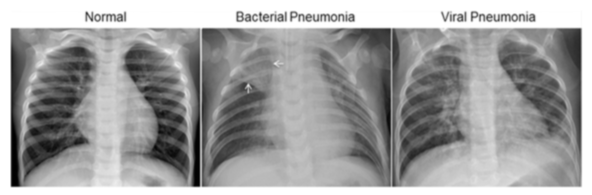
\includegraphics[width=\linewidth]{figures/Kaggle_x_ray_example.png}
  \caption{Exemplary x-ray images from the data set} 
  \label{fig:kagglePneumonia}
\end{figure}

The dataset is split into the train, validation and test set. The images were classified by two expert physicians and cleaned for low quality or unreadable scans. Additionally, the test set was verified by a third expert.
\subsection{Data Exploration}
The dataset contains 5,863 images in total. The dataset was split in a training, validation and test set from the provider of the dataset. Of those 5,863 images, 5,216 are in the training set, 16 in the validation set and 624 in the test set. Why the provider of the dataset has chosen this particular data split is unclear. 

\begin{figure}[h]
  \centering
  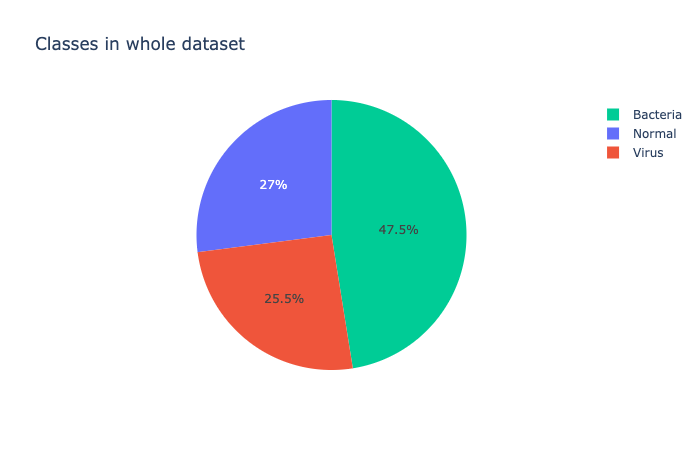
\includegraphics[width=\linewidth]{figures/pieChartClasses.png}
  \caption{Pie Chart of Classes in Data Set}
  \label{fig:data}
\end{figure}

Not only is the validation set with 16 images extremely small, which will likely cause problems, but the dataset’s classes are imbalanced as can be seen in figure \ref{fig:data}. 47.5\% of all classes in the dataset are a bacterial pneumonia infection, 25.5\% are labeled as a viral infection and 27\% have no condition. 